\documentclass{article} % For LaTeX2e
\usepackage{nips13submit_e,times}
\usepackage{hyperref}
\usepackage{url}
\usepackage{graphicx}
\usepackage{amsmath}
\usepackage{amsfonts}
%\documentstyle[nips13submit_09,times,art10]{article} % For LaTeX 2.09


\title{Modifying Spacially Correlated Training Data for Restricted Boltzmann Machines Using Integrated Nested Laplacian Approximations}


\author{
Matthew C.~Scicluna\\
Department of Statistical Sciences\\
University of Toronto\\
Toronto, ON M5S 1A1 \\
\texttt{scicluna@utstat.utoronto.ca}
}

\newcommand{\fix}{\marginpar{FIX}}
\newcommand{\new}{\marginpar{NEW}}

\nipsfinalcopy % Uncomment for camera-ready version

\begin{document}


\maketitle

\begin{abstract}
We explored using Integrated Nested Laplacian Approximation (INLA) to model handwritten digits. We trained Restricted Boltzmann Machines (RBMs) to classify these digits and compared the results of the classifier trained on the original data and on the data modified using  reconstructions from INLA. We then trained a classifier on both the aforementioned training sets taken together as a larger training set. We finally explored using the reconstruction as a starting point for training the weights of the RBM. We found that we could improve model performance by training the model on the larger training set or by using the reconstruction as a starting point- but not both. We conclude by speculating on future extensions of this approach and possible future applications.
\end{abstract}

\section{Introduction}

Gaussian Fields (GFs) are the premier statistical tool for statistical modelling of a broad class of problems [1]. There have been recent advancements in exploiting a link between GFs with Matern covariance and Gaussian Markov Random Fields (GMRFs) [2]. The details for this link are described in detail in [2], and so we will restrict our discussion henceforth to include the Matern covariance assumption insofar as to clarify it for the astute reader.

Upon making the assumption of Matern covariance we can extend Bayesian inference methodology that would otherwise be reserved for GMRFs into the broader class of GFs. In specific, we use INLA to model the data upon making the Matern covariance assumption. INLA was developed by Havard Rue and Sara Martino at the Norwegian University of Science and Technology in 2009. It is currently growing in popularity as a faster and more stable alternative to Markov Chain Monte Carlo (MCMC). 

We briefly describe the INLA methodology in the methods section, and direct the astute reader to [1] for more details. We use INLA to model training data and computed a weighted average of the training data with its reconstruction from INLA. This is thought to bring out the spacial correlations in the data to allow learning algorithms to model them more accurately. We note that the weighting average is governed by a hyperparameter $\alpha$, which represents the proportion of the weighted average that the INLA reconstruction contributes.

As a proof of concept we trained seperate Restricted Boltzmann Machines (RBMs) on a subsection of the MNIST dataset of handwritten digits described in [3]. The task was to train an RBM to be able to discriminate between the digits 3 and 5. Firstly, we used Empirical Bayes to find a suitable value for $\alpha$. We the compared the accuracy of identically configured but seperately trained RBMs to see if modifying the training data inputted in one of them (using our optimal $\alpha$) would improve its classification rate. 

We then trained a seperate RBM using both datasets to see if this approach can be benefitial in generating additional training data to learn from. This is of interest since many real-world machine learning tasks are faced with the problem of small training sets [4]. Finally, we used the inferred means of the spacial random effects as the initial weights of the RBM. We trained the data once more and compared the results.

\section{Methods}

We proceed to describe the software used and the training and test sets. We then describe the model we used for the digits, and then very briefly the INLA methodology.

\subsection{Hardware and Software Used}
All computations were done on a Sony VAIO laptop (with Intel Core i5-3337U CPU, 1.80 GHz, 8GB of RAM). The programming was done exclusively in the R programming language. The RBMs were trained using the \texttt{darch} R package. The architecture and implementation of the RBMs was based on previous research from [5]-[7]. The INLA computations were carried out using the \texttt{INLA} R package described in [8]. We note that it took approximately 4.5 minutes to run the INLA function on our machine.

\subsection{Training and Test Sets}
The training and test sets were a subsection of the MNIST dataset of handwritten digits described in [3] and which were provided by Ruslan Salakhutinov. These sets contained only instances of the digits 3 and 5. We had 400 instances of each class for the training set and 200 instances of each class for the test set.

Given our original training set $\{ Y_1, ... Y_n \}$ Let $\hat{Y}_i = \alpha Y_i + (1-\alpha) Y_i^{INLA}$ be the modified data point. $Y_i^{INLA}$ is the reconstruction of the data from INLA and $\alpha$ is the weighting average. We have that $\alpha = 0$ means that only the INLA representation contributes to the final data point and $\alpha = 1$ means that only the original data contributes. We note that this is in effect superimposing the pixels of $Y_i$ and $Y_i^{INLA}$ atop eachother.


\subsection{INLA Methodology}

We note that as of now INLA is being applied to a wide range of problems, including image analysis and spacial statistics [8] and spatio-temporal data [9]. The researchers claim, to the best of their knowledge, to be the first to use INLA in the modification or generation of training data.

We now describe in some detail the INLA methodology in regards to the specific application of modelling hand written digits described in this paper.

\subsubsection{The INLA Model}
We begin this discussion by describing the GF model provided to INLA. Given a dataset $\{ Y_1, ... , Y_n \}, Y_i \in \mathbb{R}^{8 \times 8}$ with spacial effects given by corresponding $\{ U_1, ... , U_{8 \times 8} \}$ with $d_{ij} = d(U_i, U_j)$:
\begin{enumerate}
\item[$\circ$]
    \text{Cov}$(U_i,  U_j)
    \propto
    \left(\kappa\, {d_{ij}}\right)^{\nu}
    \;
    K_{\nu}( \kappa d_{ij})$ $\leftarrow$ where $K_{\nu}$ is the modified Bessel function.


\item[$\circ$] $Y_i \sim f(\lambda_i, \theta) \leftarrow \theta$ is the range hyperparameter, a function of $\nu$ and $\kappa$.
\item[$\circ$] $g(\lambda_i) = \nu_i \leftarrow$ usually g is a log trasformation but is the identity in our model.
\item[$\circ$] $\nu_i \sim N( X_i \beta + A_i^{T}U, \tau^{-1}) \leftarrow$ We note that there is no $\beta$ (fixed effects) in our model.
\item[$\circ$] $\beta, U \sim Normal$
\item[$\circ$]
$\begin{pmatrix}
\nu \\ 
\beta \\ 
U
\end{pmatrix}$   
$\mid \theta \sim MVN \bigg( 0, \Gamma(\theta) \bigg) \leftarrow \Gamma(\theta)$ large but sparse
\end{enumerate}

We note that we can use an approximate stochastic weak solution to linear stochastic partial differential equations (SPDEs) to provide a link between between GFs with Matern covariance and GMRFs, formulated as a basis function representation. For a detailed discussion see [2].

\subsubsection{Steps INLA Takes to Compute Marginals}
INLA computes the posterior distributions of the random variables by the following steps:
\begin{enumerate}
\item Create Laplace approximation for $P(\nu, \beta, U \mid \theta, Y)$
\begin{itemize}
\item[$\circ$] should be \emph{almost} Gaussian since $P(\nu, \beta, U \mid \theta)$ is
\end{itemize}
\item Approximate marginal $P(\theta \mid Y)$
\item Integrate $\theta$ out
\item Approximate marginals $P(\beta \mid Y), P(\nu \mid Y), P(U \mid Y)$
\end{enumerate}

We direct any inclined reader to read [1] for a complete view of the method.

\section{Results}

\subsection{Comparing Averaged Data With Original}
In figure 1 we plotted some examples of the digits before and after averaging (with $\alpha=0.5$ here). We notice that they have subtle but nontrivial differences, mainly around the edges of the digits. We also see the reconstruction of the data from INLA, which has highest intensity (darkest colour) in local patches with strong variability. This is since it is modelling the dependencies between the digits. We see that averaging pronounces the local dependencies of the pixels, thus thickening the contours of the the digit and smoothing any irregularities along the edges. We can also see that this can "reconnect" any discontinuities in the digit, as can be seen in the 3 on the bottom righthand side of figure 1. To further this point we vary the value of $\alpha$ and plot it in figure 2.

\begin{figure}[h]
\begin{center}
  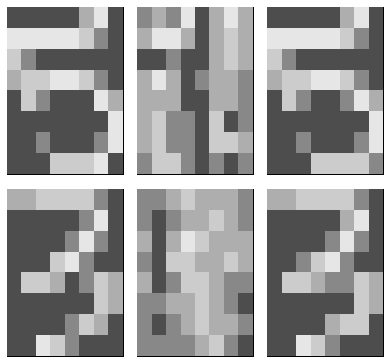
\includegraphics[width=50mm]{figures/Rplotgood.png}
\end{center}
\caption{Comparing a representative digit from each class (left), the INLA representation (centre) and the average of the two (right)  }
\end{figure}

\begin{figure}[h]
\begin{center}
  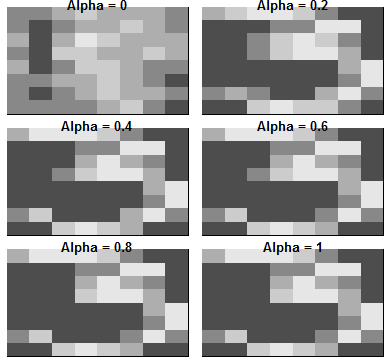
\includegraphics[width=50mm]{figures/Rplot22.png}
\end{center}
\caption{Comparing a representative digit from the 3 class upon varying the value of alpha}
\end{figure}


\subsection{Comparing RBMs Trained With Averaged Data VS Trained With Only Original Data}

We used Empirical Bayes to optimize over the hyperparameter $\alpha$. We left out a quarter of the data from the training set to use as a validation set and performed a grid search of $\alpha$ within the unit interval. Our objective function was the validation error rate. We plotted the effect of $\alpha$ on this objective function in figure 3. Note that we did not apply the averaging to the validation data, only to the training data. This is since our aim is to predict the original data and not the modified data. For each value of $\alpha$ we trained 5 seperate models and averaged the resultant 5 validation error rates to control for variability between models. We found that $\alpha = 0.9$ gave the best performance, meaning that it was best to only add a small contribution from the INLA reconstruction.


\begin{figure}[h]
\begin{center}
  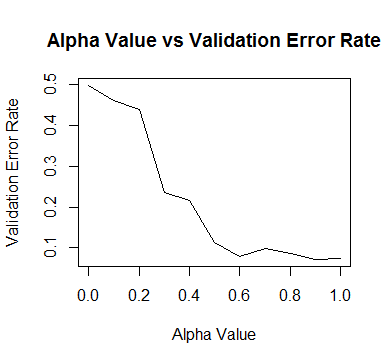
\includegraphics[width=75mm]{figures/Rplot33.png}
\end{center}
\caption{Comparing the error rate of the data as a function of alpha}
\end{figure}

Using the optimal $\alpha$, we trained 5 seperate models with the modified data and 5 with the original data and compared the average test error, again to control for model variability. We found that the model trained on the original data slightly outperformed the model trained on the modified training data, although the difference was within the margin of error. The results are presented in Table 1.

\subsection{Comparing RBMs Trained With Both Averaged Data And Original Data}

We then explored training an RBM on both the original and averaged data. We found that the test error rate decreased to 5.6\%. Since the model seemed to be unable to distinguish the digit with its averaged representation we see that we essentially doubled the training data of the model while maintaining the models capacity. We note that this is not equivalent to bagging since the new data is not identical to the old and is not being sampled from. The results can be found in Table 1.

\begin{table}[t]
\caption{Results of Experiment}
\label{sample-table}
\begin{center}
\begin{tabular}{ll}
\multicolumn{1}{c}{\bf TRAINING DATA USED}  &\multicolumn{1}{c}{\bf TEST ERROR RATE (\%)}
\\ \hline \\
Without Averaging         &7.3 $\pm$ 1.3\\
Without Averaging But With Initialization & 5.8 $\pm$ 0.73\\
With Averaging And Initialization & 7.55 $\pm$ 0.9\\
With Only Averaging             & 7.55 $\pm$ 1.4 \\
With Both Types of Data            & 5.6 $\pm$ 1.1 \\
\end{tabular}
\end{center}
\end{table}


\subsection{Using INLA Representation As Initialized Weights}
Finally, we experimented with using the mean of the random effects in the GF as initialization weights for each of the hidden units of the RBM. We found that this sped up training and improved model performance, although the effect diminished if we used the averaged data instead of the original. Again the results are summarized in Table 1. 

\section{Conclusions}

While we did not find that the model improved upon modifying the data, we did find an improvement by setting the weights to the learned values of the random effects from the INLA model.

We also found that using the averaged data along with the original data improved model accuracy in this task, indicating that this method is viable as a technique to produce new "pseudo-data" for training purposes. Using INLA for this application has the added benefit that computations are comparitively faster and more numerically stable than more popular alternatives like MCMC [1].

\subsection{Future Directions}
We speculate that this technique can be further modified to produce even more "pseudo-data" for training purposes. We can explore adjusting the hyperparameters of the Matern covariance or consider other covariance structures altogether (albeit with no guarentee INLA will be able to model it). We also propose that the above method could be used as a new imputation technique for missing data or for data with occlusion, due to its generative nature.

\subsection{Acknowledgments}

We would like to thank Professor Richard Zemel for his excellent instruction throughout the term as well as for the teaching assistants  which led very informative tutorials. Finally we would like to thank Wenjie Luo for the advice he provided in the writing of this paper.

\subsubsection*{References}

\small{

[1] Rue, H. \& Martino, S. (2009) Approximate Bayesian inference for latent Gaussian models by using integrated nested Laplace approximations. {\it Journal of the Royal Statistical Society: Series B (Statistical Methodology)}
{\bf 71}(2): 319 - 392.

[2] Rue, H. \& Lindgren, F. (2011) An Explicit Link Between Gaussian Fields and
Gaussian Markov Random Fields: The SPDE Approach. {\it Journal of the Royal Statistical Society: Series B (Statistical Methodology)}
{\bf 73}(4): 423 - 498.

[3] LeCun, Y.,  Bottou, L.,  Bengio Y. \& Haffner, P. (1998) Gradient-Based Learning Applied to Document Recognition. {\it Proceedings of the IEEE} {\bf 86}(11) 2278 - 2324.

[4] Forman, G. \& Cohen, I. (2004) Learning from Little: Comparison of Classifiers Given Little Training. {\it Lecture Notes in Computer Science} {\bf 3202}: 161-172.

[5] Hinton, G., Osindero, S. \& Teh, Y. (2006) A fast learning algorithm for deep belief nets. {\it Neural Computation} {\bf 18}(7): 1527 - 1554.

[6] Hinton, G \&  Salakhutdinov, R. (2006) Reducing the Dimensionality of Data with Neural Networks. {\it Science} {\bf 313}(5786): 504 - 507.

[7] Hinton, G (2002) Training products of experts by minimizing contrastive divergence. {\it Neural Computation} {\bf 14}(8): 1771 - 1800.

[8]  Lindgren, F. \& Rue, H. (2015) Bayesian Spatial Modelling with R-INLA. {\it Journal of Statistical Software} {\bf 63}(19): 1 - 29.

[9] Blangiardo, M. (2013) Spatial and spatio-temporal models with R-INLA. {\it Spatial and Spatio-temporal Epidemiology} {\bf 4}: 33-49.
}

\end{document}
